\documentclass[11pt, a4paper]{article}
\usepackage[affil-it]{authblk} 
\usepackage{etoolbox}
\usepackage{lmodern}
\usepackage{titlesec}
\usepackage{float}

\makeatletter
\patchcmd{\@maketitle}{\LARGE \@title}{\fontsize{20}{19.2}\selectfont\@title}{}{}
\makeatother

\renewcommand\Authfont{\fontsize{16}{14.4}\selectfont}
\renewcommand\Affilfont{\fontsize{12}{10.8}\itshape}

\title{\textbf{Endsem}} 
\author{Pavan R Hebbar - 130010046}
\usepackage{graphicx}
\begin{document}
\maketitle
\newpage
\section{Question 1:}

The plasma parameters for various palsmas have been shown below. The x axis corresponds to the number 
of the length scale in the question. 
\begin{figure}[H]
 \centering
 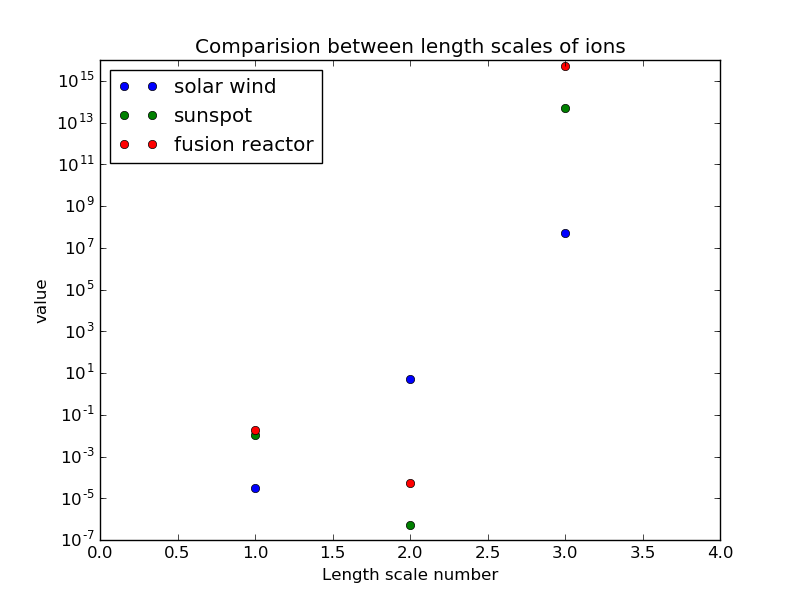
\includegraphics[scale = 0.6]{ques1_len.png}
 \caption{Plasma length scales for ions}
\end{figure}

The xaxis corresponds to the timescale no. in the question
\begin{figure}[H]
 \centering
 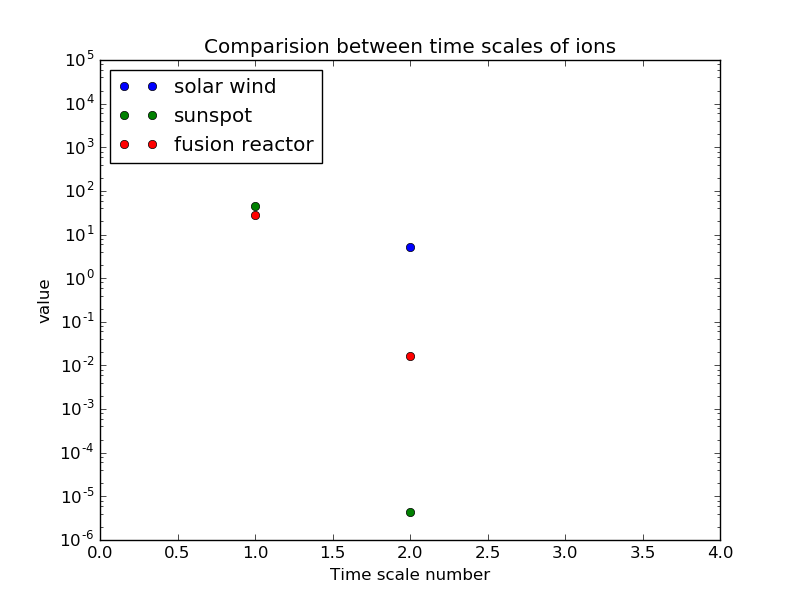
\includegraphics[scale = 0.6]{ques1_time.png}
 \caption{Plasma time scales for ions}
\end{figure}

\begin{figure}[H]
 \centering
 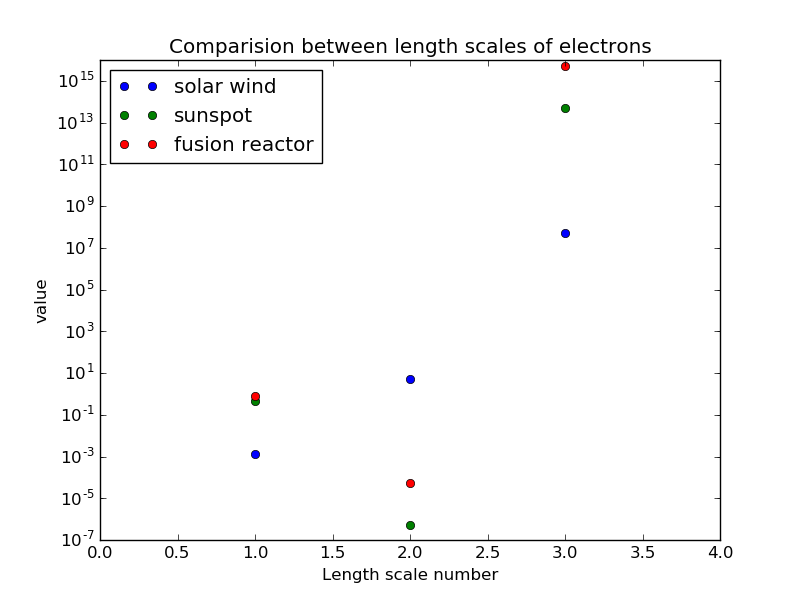
\includegraphics[scale = 0.6]{ques1_len2.png}
 \caption{Plasma length scales for electrons}
\end{figure}

The xaxis corresponds to the timescale no. in the question
\begin{figure}[H]
 \centering
 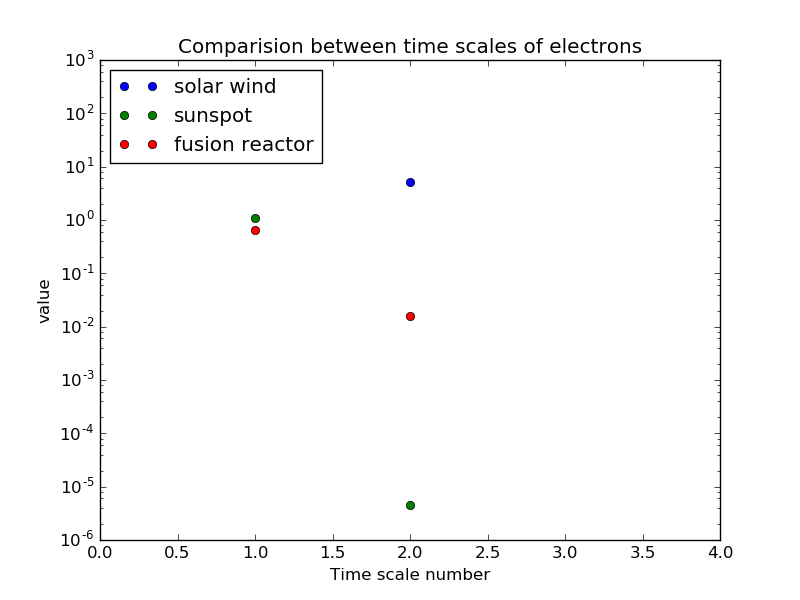
\includegraphics[scale = 0.6]{ques1_timee.png}
 \caption{Plasma time scales for electrons}
\end{figure}

\section{Question 2:}
\subsection{a)}
As shwn in the calculations in the answer sheet we see that the magnetic moment is in fact a adiabatic invariant.
This can be seen even in the simulation when where is no electric field. We see that the relative error is of the order of $10^-12$ which is negligible
\begin{figure}[H]
 \centering
 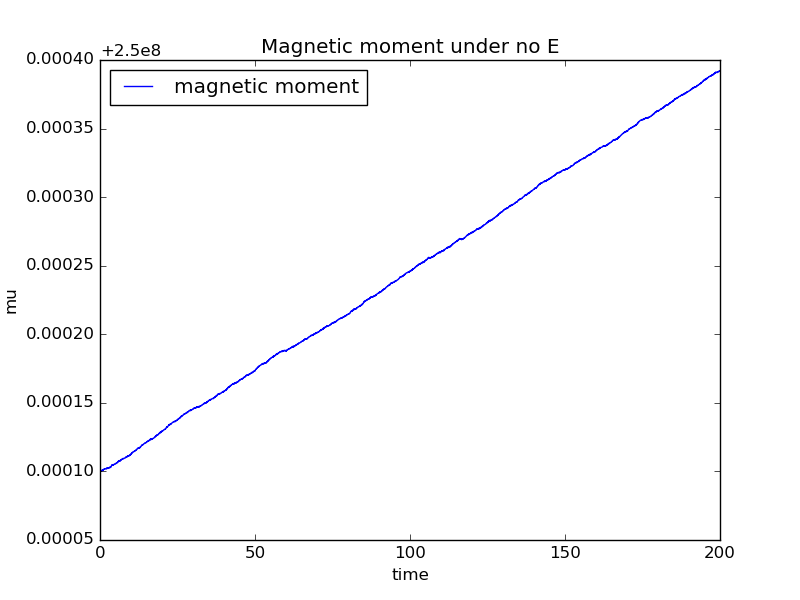
\includegraphics[scale = 0.6]{ques2a_1.png}
 \caption{Variation of magnetic moment}
\end{figure}
When there is a constant electric field of $10^5N/m$, we see that $\mu$ oscillates
\begin{figure}[H]
 \centering
 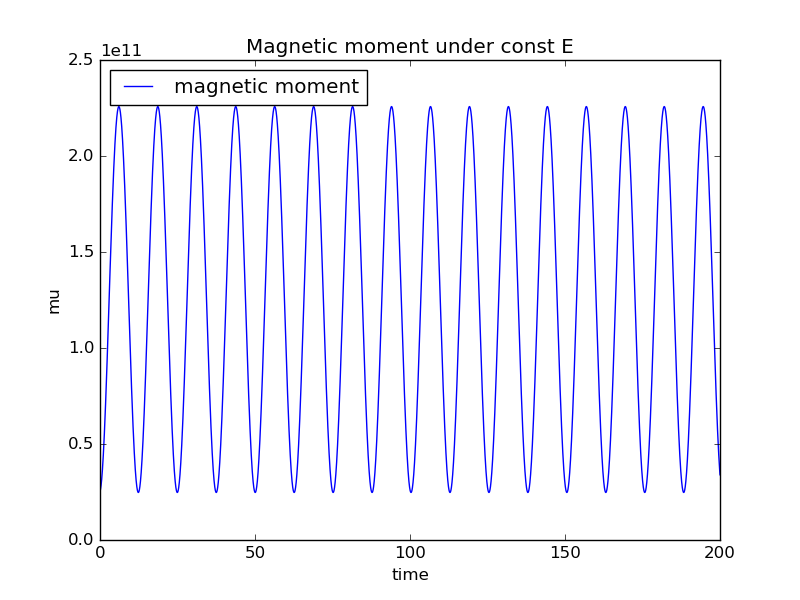
\includegraphics[scale = 0.6]{ques2a_2.png}
 \caption{Variation of magnetic moment}
\end{figure}

\subsection{b)}:
On solving we get the analytical solution as worked out in the answer booklet. For simulation we used the amplitude of electric field as $10^5$
and the frequency as 0.2
\begin{figure}[H]
 \centering
 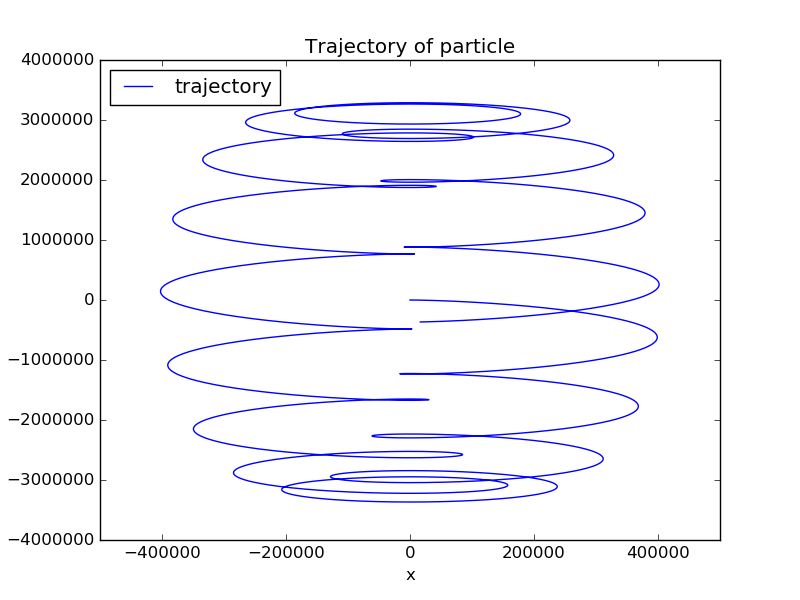
\includegraphics[scale = 0.6]{ques2b_pos.png}
 \caption{Change in position}
\end{figure}

\begin{figure}[H]
 \centering
 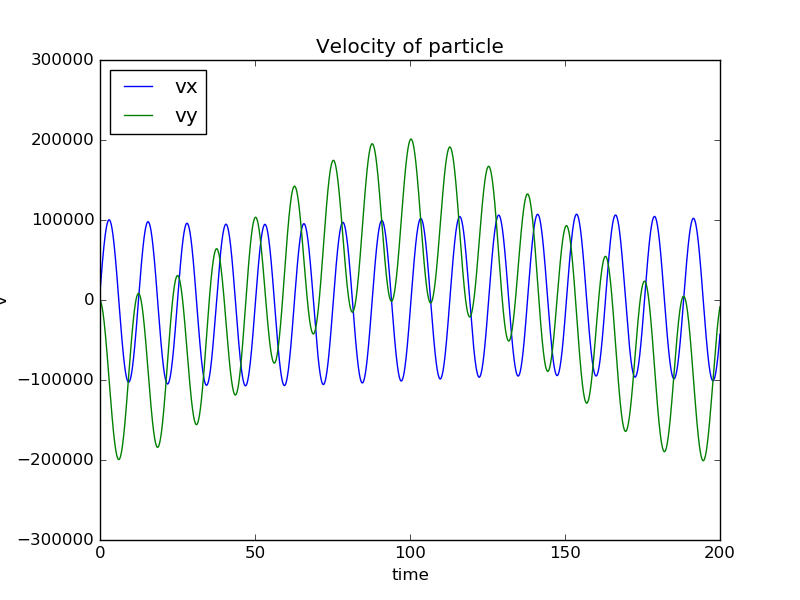
\includegraphics[scale = 0.6]{ques2b_vel.png}
 \caption{Change in velocity}
\end{figure}
We see that the change in vx and vy is similar to addition of 2 sine waves which is similar to the nature of the analystical solution
(Some problem with the implementation of the exact soln, therefore not able to find the error)
Also, since the electric field is oscillating it increases the random motion of the particles. This the conductivity decreases
\subsection{c)}
Electric field of 10 V/m was used to simulate the result.
\begin{figure}[H]
 \centering
 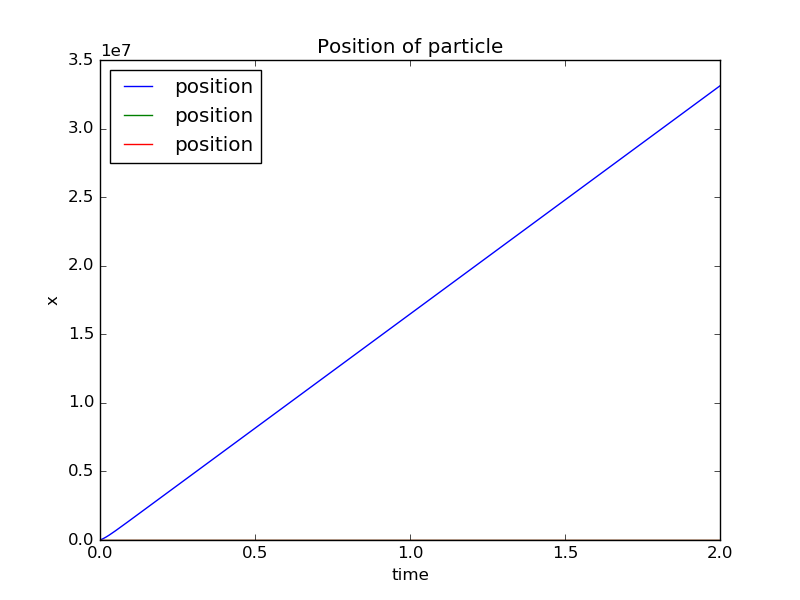
\includegraphics[scale = 0.6]{ques2c_pos.png}
 \caption{Change in position}
\end{figure}
Since the particle density of the plasma is high and the temperature is cold, the conductivity of this plasma would be much more than its surroundings


\begin{figure}[H]
 \centering
 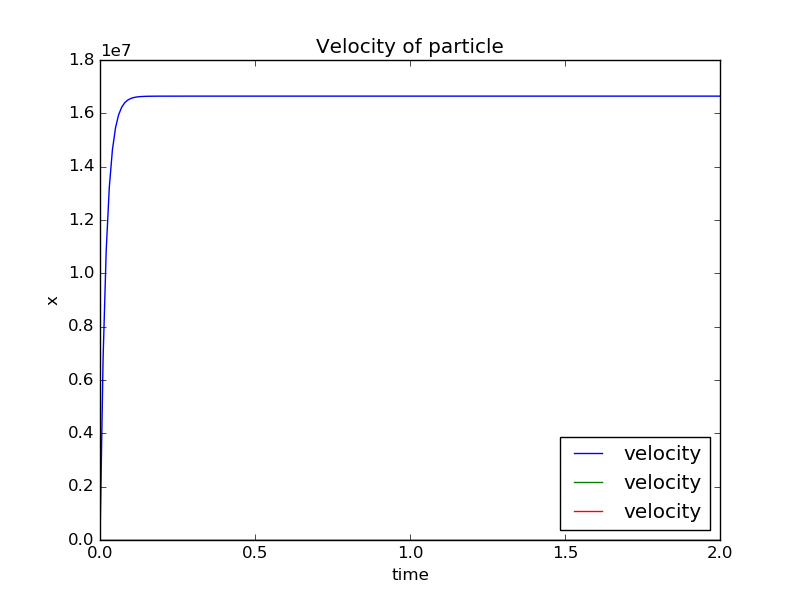
\includegraphics[scale = 0.6]{ques2c_vel.png}
 \caption{Change in velocity}
\end{figure}
\end{document}